\documentclass[11pt]{article}
\usepackage[margin=1in]{geometry}
\usepackage{graphicx}
\usepackage{booktabs}
\usepackage{amsmath,amssymb}
\usepackage{hyperref}
\usepackage{caption}
\usepackage{subcaption}
\usepackage{multirow}

\title{Gaussian Mutual Information Analysis of Transformer MLP Layers:\\
Empirical Evidence for the Information Bottleneck in Pretrained LLMs}
\author{Fergie (Yishu) Yang}
\date{May 5, 2026}

\begin{document}
\maketitle

\begin{abstract}
We compute the Gaussian mutual information (MI) between each transformer layer's MLP output and the final layer's MLP output across four pretrained language models (0.6B--1.7B parameters). Combined with the effective rank analysis from our team's earlier pipeline, this provides both axes of the Information Bottleneck (IB) information plane: effective rank as a proxy for $I(T;X)$ (representation complexity) and Gaussian MI as a proxy for $I(T;Y)$ (informativeness). We report five findings: (1)~MLP output MI exhibits a universal two-phase pattern---flat plateau followed by exponential rise---with sharp drops at near-rank-1 layers; (2)~residual stream MI is smooth and monotonically increasing, consistent with the Data Processing Inequality; (3)~late layers simultaneously show declining effective rank and rising MI, consistent with the IB compression--informativeness tradeoff; (4)~these patterns are universal across all four architectures; (5)~information density $\ln(\mathrm{MI}/\mathrm{Rank})$ follows a U-shaped curve across depth, revealing that rank-1 layers are not redundancies but learned bottlenecks with maximal information concentration, and that only 2--4 layers per model are Pareto-efficient in the complexity--informativeness plane. These patterns emerge from standard pretraining without any IB-explicit training objective.
\end{abstract}

%% ================================================================
\section{Motivation and Logical Chain}
%% ================================================================

The Information Bottleneck principle \cite{tishby2015} characterizes each layer's representation $T_\ell$ by two quantities:
\begin{itemize}
    \item $I(T_\ell; X)$: how much the representation preserves about the input (\emph{complexity}).
    \item $I(T_\ell; Y)$: how much the representation captures about the target (\emph{informativeness}).
\end{itemize}
Optimal representations maximize informativeness for a given complexity budget, tracing the IB curve in the $(I(T;X),\, I(T;Y))$ information plane.

Our team's earlier pipeline computes \textbf{effective rank}---the exponential of spectral entropy of the MLP output covariance---as a proxy for $I(T;X)$. This gives us the complexity axis. My contribution is the second axis: \textbf{Gaussian mutual information} between each layer and the final layer, providing a proxy for $I(T;Y)$.

The logical chain is:
\begin{enumerate}
    \item Effective rank tells us \emph{how complex} each layer's representation is.
    \item Gaussian MI tells us \emph{how informative} each layer's representation is about the model's output.
    \item Together, they place each layer in the IB information plane.
    \item If the IB principle governs trained LLM representations, we expect late layers to \emph{compress} (declining rank) while becoming \emph{more informative} (rising MI).
    \item We test this prediction across four architectures.
\end{enumerate}

%% ================================================================
\section{Method}
%% ================================================================

\subsection{Setup}

We analyze four models on 65,536 token activations from WikiText-2:

\begin{table}[h]
\centering
\begin{tabular}{lccc}
\toprule
\textbf{Model} & \textbf{Parameters} & \textbf{Layers} & \textbf{Hidden dim} \\
\midrule
Qwen3-0.6B & 0.6B & 28 & 1024 \\
Qwen2.5-1.5B & 1.5B & 28 & 1536 \\
SmolLM2-1.7B & 1.7B & 24 & 2048 \\
Llama-3.2-1B & 1.0B & 16 & 2048 \\
\bottomrule
\end{tabular}
\end{table}

\subsection{Representations}

We measure MI on two representations:
\begin{enumerate}
    \item \textbf{MLP output} $\mathbf{m}_\ell$: the additive contribution of layer $\ell$'s feedforward network. This isolates what each individual MLP contributes.
    \item \textbf{Residual stream} $\mathbf{h}_\ell$: the full hidden state after layer $\ell$, accumulating all prior contributions via skip connections.
\end{enumerate}

\subsection{Gaussian MI Computation}

We compute $I(\mathbf{m}_\ell;\, \mathbf{m}_L)$ for MLP outputs and $I(\mathbf{h}_\ell;\, \mathbf{h}_L)$ for residual streams, under the assumption of joint Gaussianity, using two numerically complementary methods:

\paragraph{CCA method (primary for MLP output).}
Compute canonical correlations $\rho_i$ from the whitened cross-covariance $\Sigma_\ell^{-1/2}\,\Sigma_{\ell L}\,\Sigma_L^{-1/2}$, then:
\begin{equation}
    I_{\mathrm{CCA}} = -\frac{1}{2}\sum_{i} \log(1 - \rho_i^2)
\end{equation}
We use \emph{truncated whitening}: eigenvalues below $10^{-5}\times\lambda_{\max}$ are excluded before inversion to avoid noise amplification in the null space of near-singular covariances.

\paragraph{Log-det method (primary for residual stream).}
\begin{equation}
    I_{\mathrm{log\text{-}det}} = \frac{1}{2}\bigl(\log\det\Sigma_\ell + \log\det\Sigma_L - \log\det\Sigma_{\mathrm{joint}}\bigr)
\end{equation}
where $\Sigma_{\mathrm{joint}}$ is the joint covariance of $(\mathbf{h}_\ell, \mathbf{h}_L)$. Regularization $\varepsilon \mathbf{I}$ ($\varepsilon = 10^{-8}$) is added for stability. Log-determinants are computed as sums of log-eigenvalues, never via $\log(\det(\cdot))$.

Both methods compute the same quantity under exact arithmetic; the choice between them is driven by numerical stability for each representation type.

\paragraph{Why Gaussian MI?}
MLP outputs pass through nonlinear activations and are not truly Gaussian. However: (i)~Gaussian MI provides a \textbf{lower bound} on the true MI (among all distributions with the same covariance, the Gaussian has minimum entropy, hence minimum MI); (ii)~non-parametric MI estimators do not scale to 1024+ dimensions with $\sim$65k samples; (iii)~the \textbf{relative ordering} between layers is reliable even under the Gaussian approximation.

%% ================================================================
\section{Finding 1: Two-Phase MLP Output MI with Rank-1 Drops}
\label{sec:f1}
%% ================================================================

\begin{figure}[h]
\centering
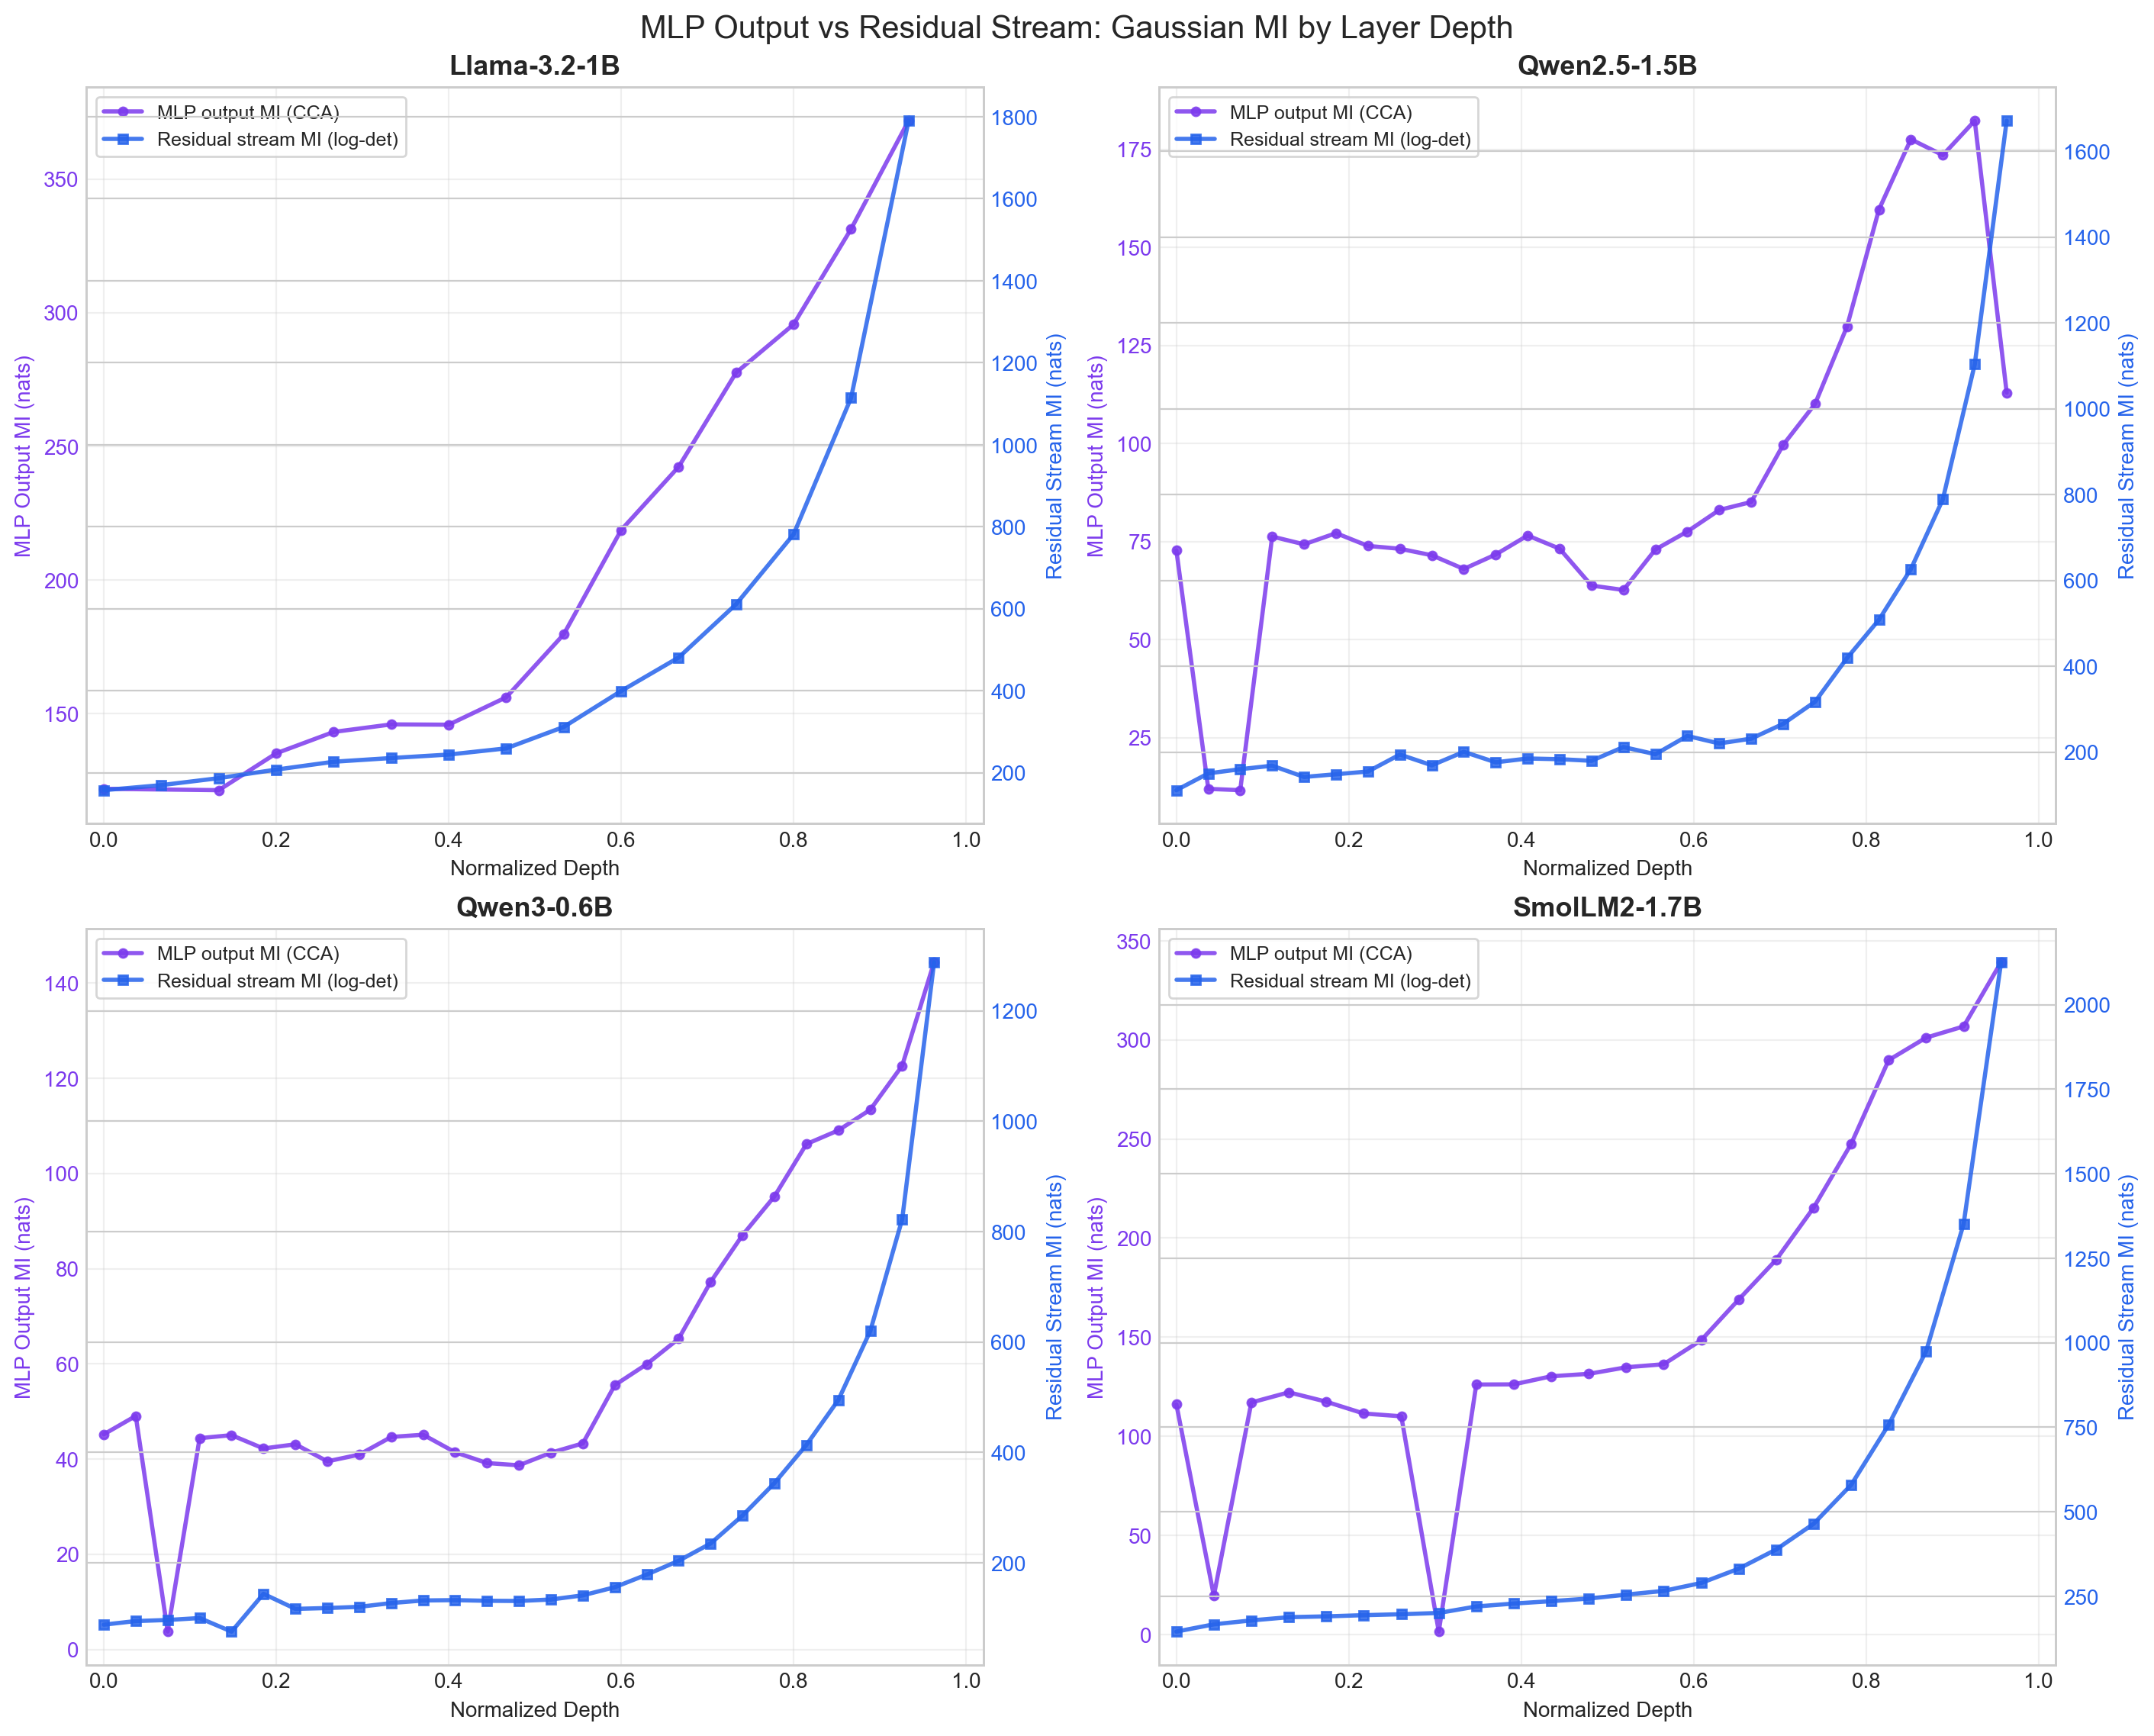
\includegraphics[width=\textwidth]{result/6c_mi_comparison/mi_mlp_vs_residual.png}
\caption{MLP output MI (purple, CCA, left $y$-axis) vs.\ residual stream MI (blue, log-det, right $y$-axis) across normalized depth for all four models. Dual $y$-axes reflect the different absolute scales.}
\label{fig:raw}
\end{figure}

Across all four models, MLP output MI shows a consistent two-phase pattern (Figure~\ref{fig:raw}, purple curves):

\begin{enumerate}
    \item \textbf{Flat plateau} (early/middle layers, $\sim$0--60\% of depth): MI fluctuates in a narrow band. These MLPs produce outputs only moderately correlated with the final layer.
    \item \textbf{Exponential rise} (late layers, $\sim$60--100\% of depth): MI increases steeply as successive MLPs become increasingly aligned with the final representation.
\end{enumerate}

\textbf{Interpretation.} Early/middle MLP layers perform broadly distributed, ``preparatory'' transformations that do not yet resemble the model's final output computation. Late MLP layers increasingly specialize toward the output, each adding representations highly correlated with the final prediction head's input.

\subsection{Rank-1 Anomaly Layers}

Every model exhibits 1--3 layers where the MLP output has \textbf{effective rank $\approx 1$}: all tokens' MLP outputs are approximately scalar multiples of a single direction. These layers produce sharp MI drops:

\begin{table}[h]
\centering
\begin{tabular}{lcccc}
\toprule
\textbf{Model} & \textbf{Layer(s)} & \textbf{Eff.\ Rank} & \textbf{CCA Dims} & \textbf{MI (nats)} \\
\midrule
Qwen3-0.6B & 2 & 1.004 & 1 & 3.75 \\
\midrule
\multirow{3}{*}{Qwen2.5-1.5B} & 1 & 1.033 & 28 & 11.9 \\
 & 2 & 1.047 & 31 & 11.6 \\
 & 26 & 1.257 & 569 & 113.0 \\
\midrule
\multirow{2}{*}{SmolLM2-1.7B} & 1 & 1.095 & 70 & 19.5 \\
 & 7 & 1.119 & 5 & 1.43 \\
\midrule
Llama-3.2-1B & 1 & 1.041 & 1442 & $\infty$ \\
\bottomrule
\end{tabular}
\caption{Near-rank-1 MLP layers. ``CCA Dims'' = dimensions surviving truncated whitening. The $\infty$ for Llama layer~1 reflects numerical instability when too many dimensions survive despite near-singularity.}
\label{tab:drops}
\end{table}

A rank-1 MLP output means the layer's feedforward contribution is essentially one-dimensional. Such a layer has minimal complexity ($I(T;X) \approx 0$), but informativeness varies with depth: early rank-1 layers (layers~1--2) carry low MI and are safely compressible, while late rank-1 layers (e.g., Qwen2.5 layer~26 with 113~nats) funnel significant output-relevant information through a single direction. As shown in Section~\ref{sec:f5}, these late rank-1 layers are among the most \emph{information-dense} representations in the network---compressing them risks substantial information loss.

%% ================================================================
\section{Finding 2: Residual Stream MI Is Smooth and Monotonic}
\label{sec:f2}
%% ================================================================

\begin{figure}[h]
\centering
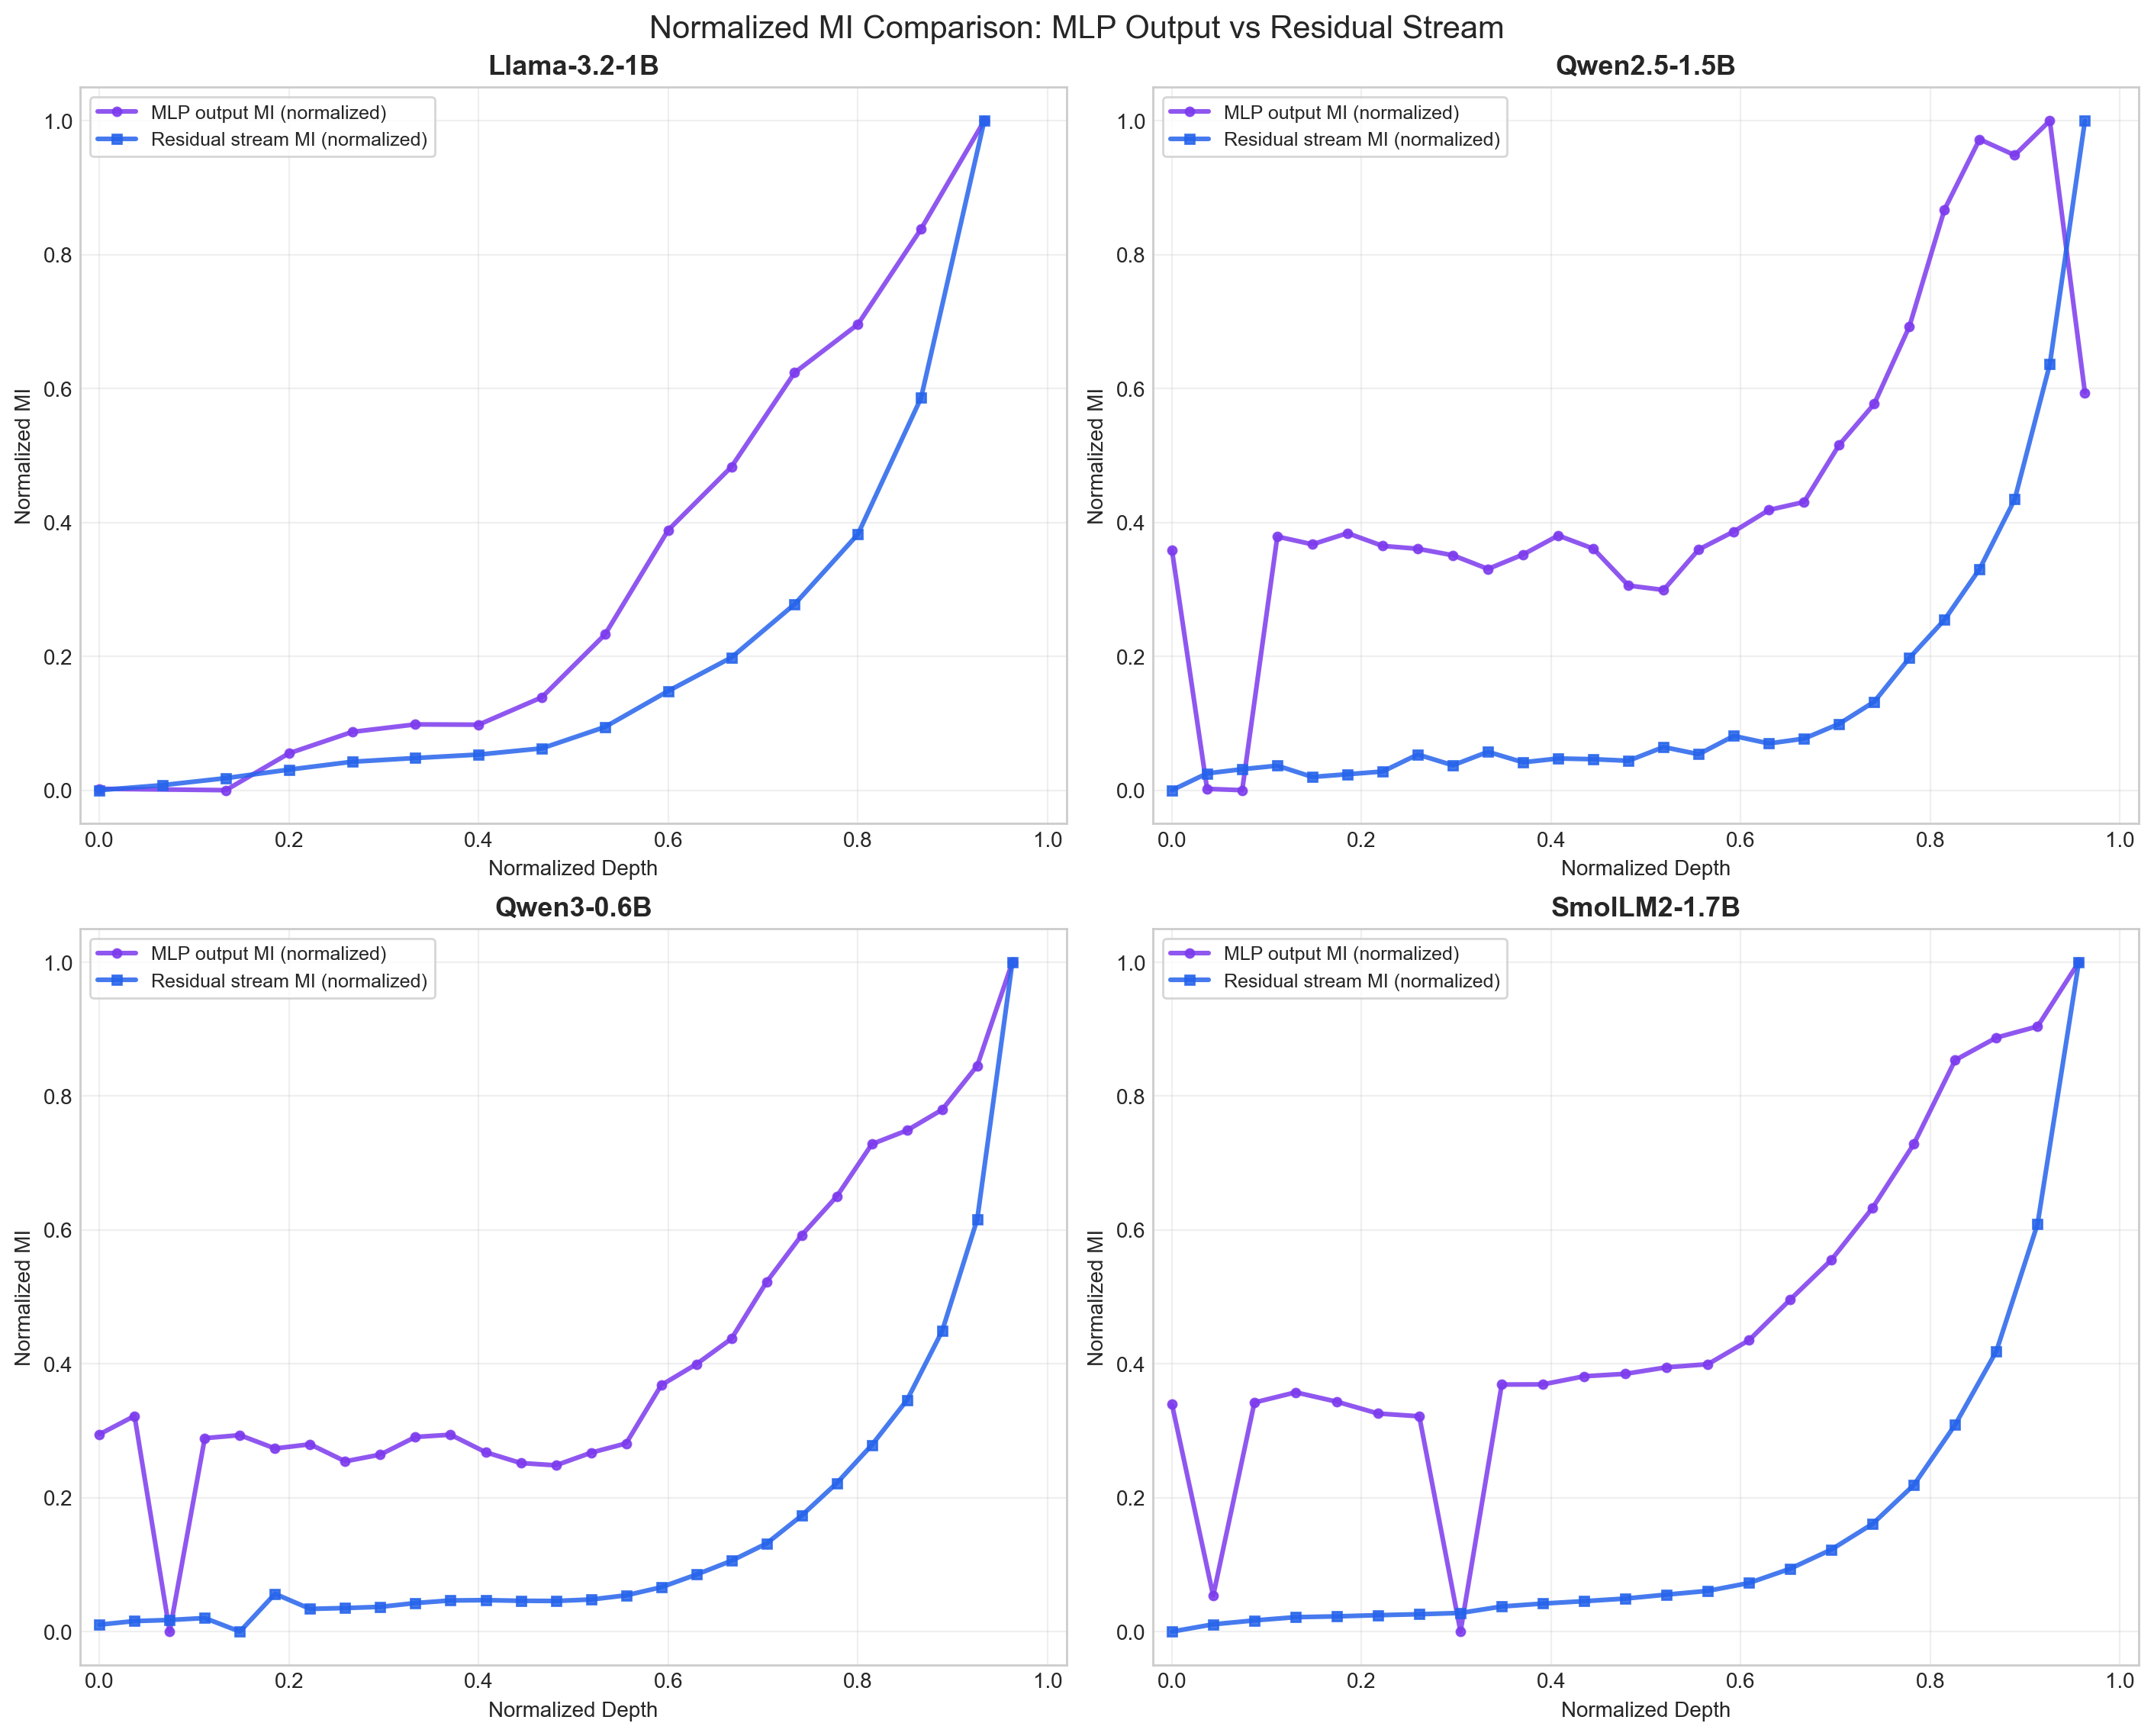
\includegraphics[width=\textwidth]{result/6c_mi_comparison/mi_mlp_vs_residual_normalized.png}
\caption{Normalized MI (min-max scaled to $[0,1]$). Purple: MLP output (CCA). Blue: residual stream (log-det). The residual stream is smooth and monotonic; MLP output shows drops and a flatter early/middle profile.}
\label{fig:normalized}
\end{figure}

The residual stream MI (blue curves in Figure~\ref{fig:raw}) is smooth and monotonically increasing for all four models. This is theoretically expected: the residual stream forms a Markov chain
\[
X \to \mathbf{h}_0 \to \mathbf{h}_1 \to \cdots \to \mathbf{h}_L
\]
and by the \textbf{Data Processing Inequality} (DPI), $I(\mathbf{h}_\ell;\, \mathbf{h}_L)$ must be non-decreasing in $\ell$.

The contrast between the two curves (Figure~\ref{fig:normalized}) reveals a per-layer decomposition:

\begin{itemize}
    \item \textbf{Low MLP MI + rising residual MI}: the layer's MLP contributes little new information; the increase comes from what was already in the residual stream via skip connections. These are \emph{redundant} MLP layers.
    \item \textbf{Sharply rising MLP MI}: the layer's MLP makes a significant new contribution. These are \emph{critical} MLP layers.
    \item \textbf{At rank-1 drop layers}: residual MI continues its smooth increase, confirming that \emph{no information is lost} at the network level---the skip connection carries everything past the degenerate MLP.
\end{itemize}

%% ================================================================
\section{Finding 3: The IB Scissors---Empirical Compression-Informativeness Tradeoff}
\label{sec:f3}
%% ================================================================

\begin{figure}[h]
\centering
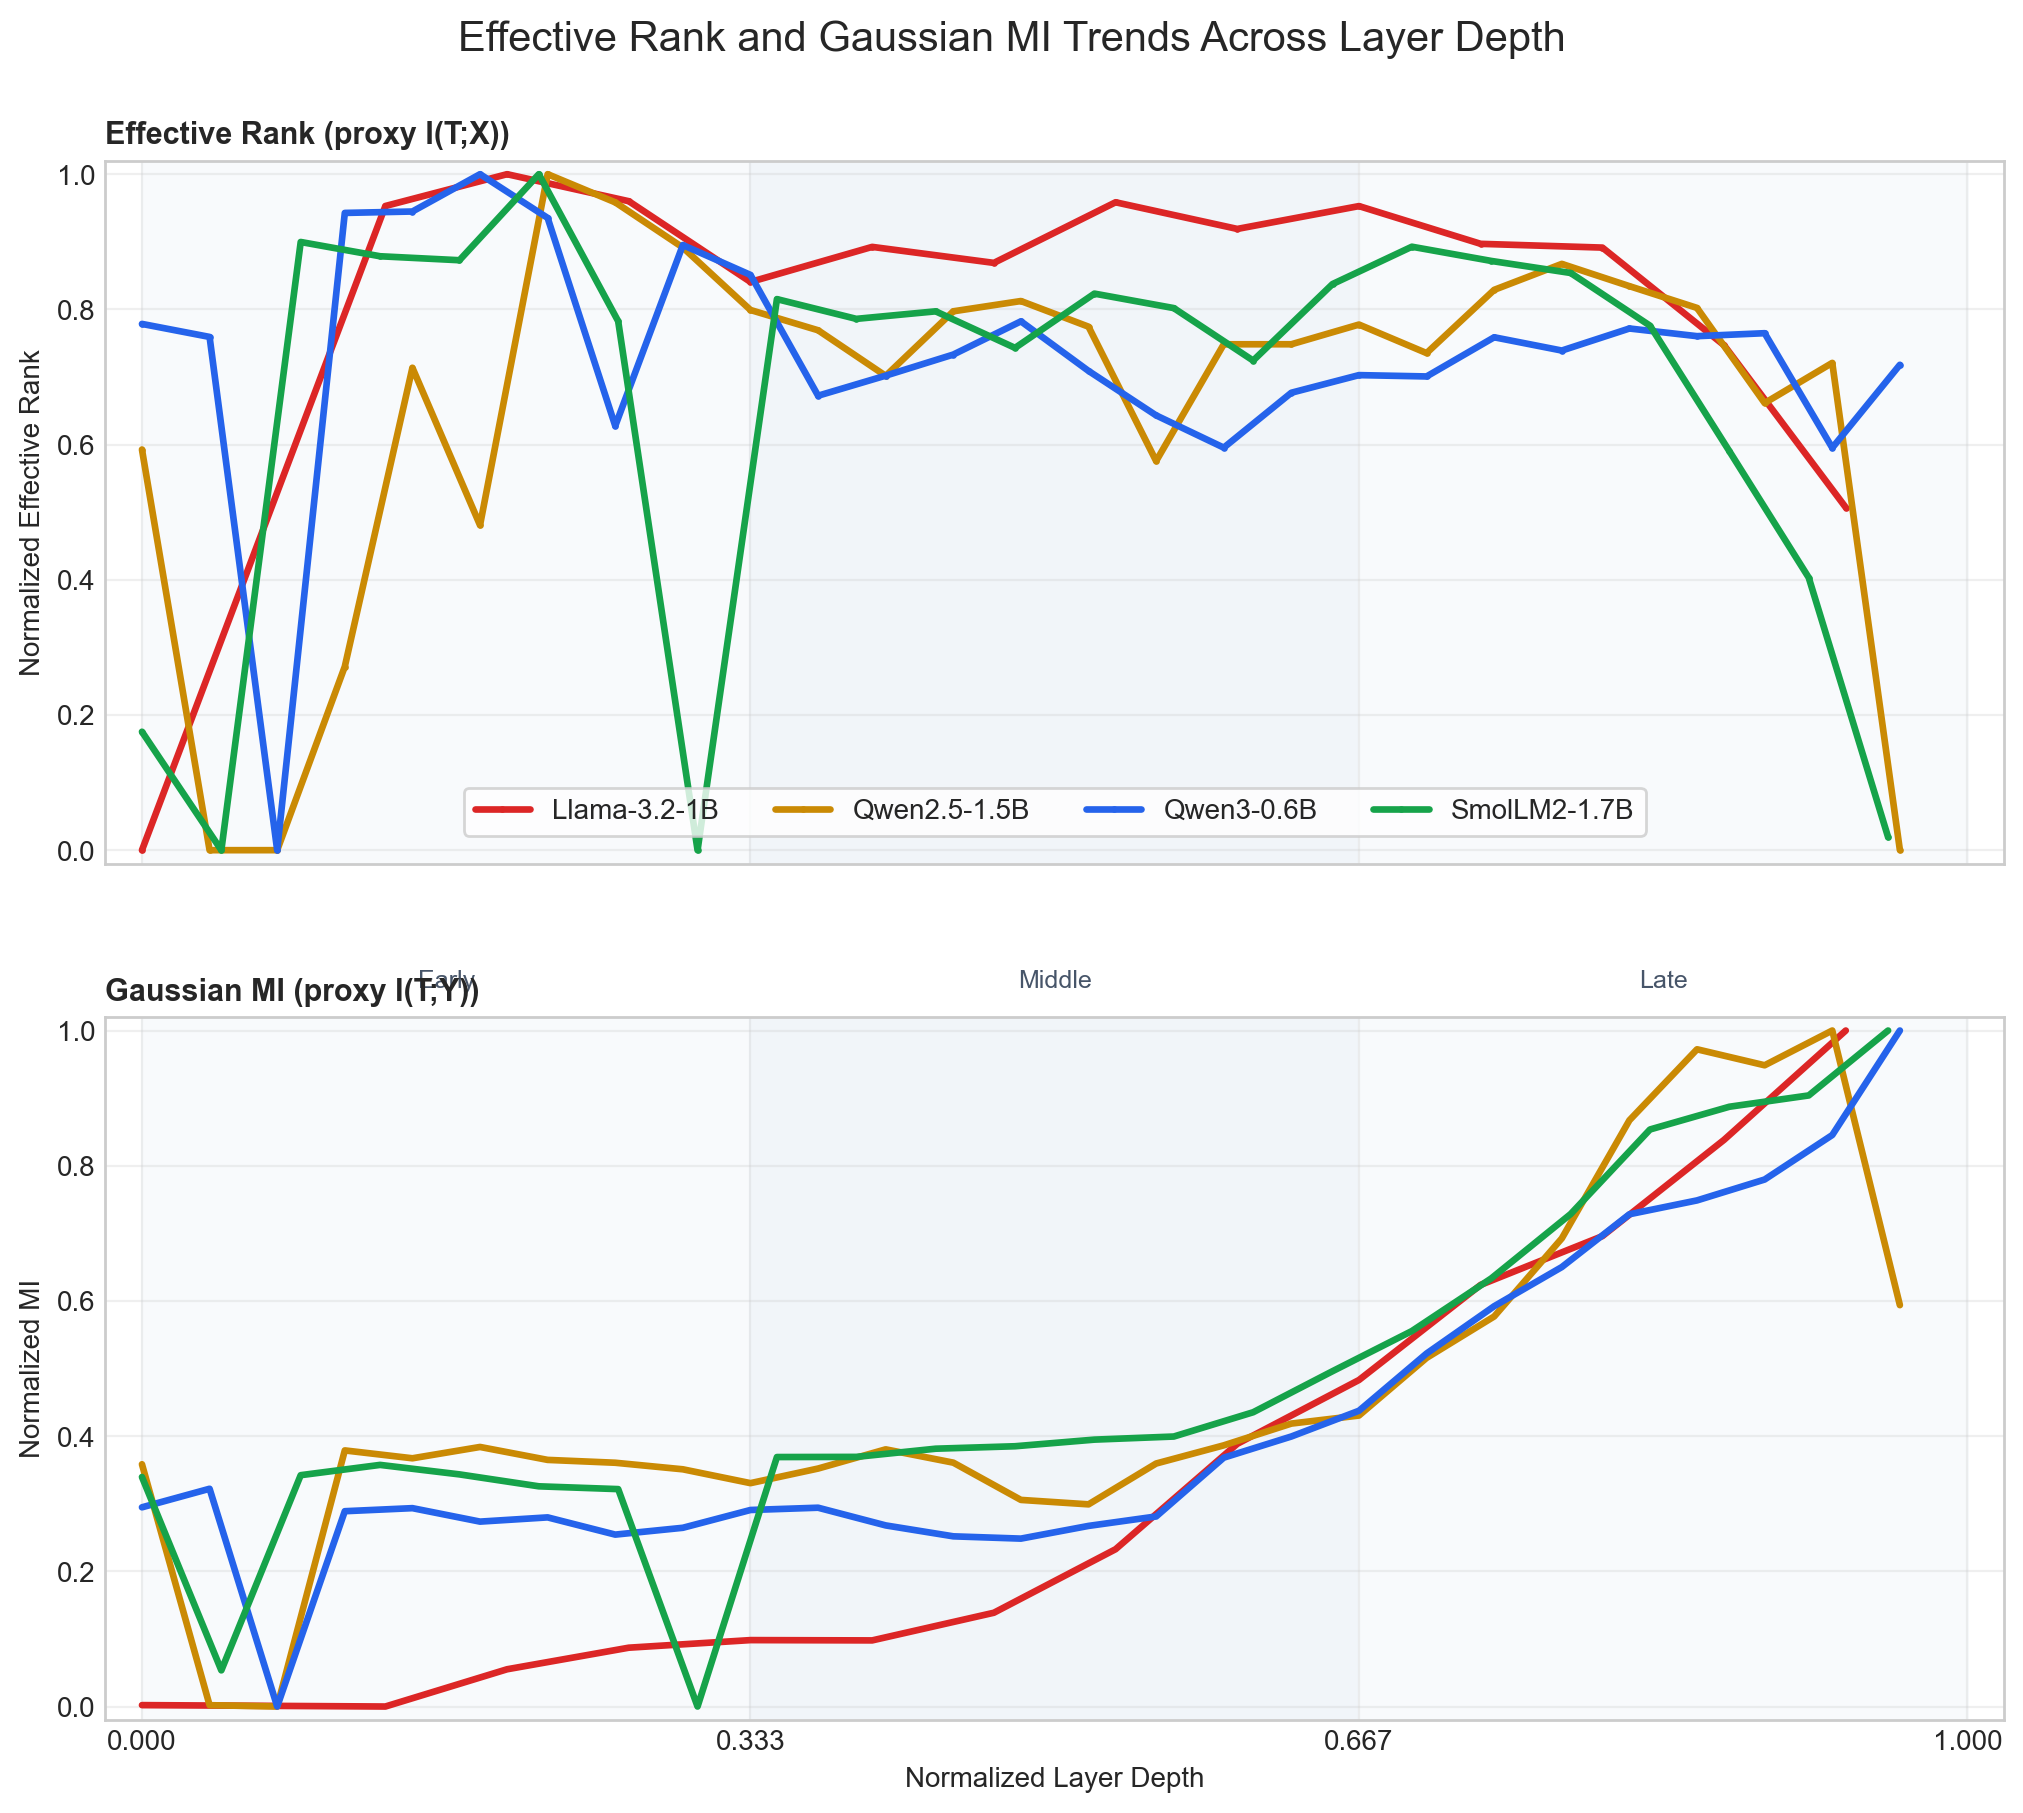
\includegraphics[width=0.85\textwidth]{result/7_information_plane/mi_rank_trends.png}
\caption{Top: normalized MLP output effective rank (proxy $I(T;X)$) across depth. Bottom: normalized Gaussian MI (proxy $I(T;Y)$) across depth. In the \textbf{Late} region (depth $> 0.667$), effective rank declines while MI rises---the IB ``scissors'' pattern.}
\label{fig:scissors}
\end{figure}

The key finding emerges from reading both axes of the IB plane together across depth (Figure~\ref{fig:scissors}):

\begin{itemize}
    \item \textbf{Late layers} (final $\sim$30\% of depth): effective rank \emph{drops} (the representation compresses into fewer effective dimensions) while MI \emph{rises} (the representation becomes more aligned with the output).
    \item This is exactly the \textbf{compression--informativeness tradeoff} predicted by the Information Bottleneck principle: optimal representations should compress the input while preserving task-relevant information.
\end{itemize}

This ``scissors'' pattern---rank declining as MI rises---is observed in all four models despite different architectures, parameter counts, and training procedures. The tradeoff is a \emph{depth-dependent trajectory} through the information plane, not a static correlation: earlier layers build up complexity (high rank, moderate MI), while later layers shed unnecessary dimensions and focus on the output.

\textbf{Why a depth-dependent trajectory, not a scatter correlation?} The IB tradeoff manifests as the \emph{direction} layers move through the information plane as depth increases. A naive scatter of rank vs.\ MI across all layers yields weak correlations ($r = 0.06$--$0.35$) because early/middle layers occupy a different regime (building up representations) than late layers (compressing toward the output). The tradeoff is visible only when we track how both quantities evolve with depth.

%% ================================================================
\section{Finding 4: Universality Across Architectures}
\label{sec:f4}
%% ================================================================

All four models---spanning three model families, hidden dimensions from 1024 to 2048, and 16 to 28 layers---share:

\begin{enumerate}
    \item \textbf{MLP output MI}: flat early/middle $\to$ exponential late growth, with 1--3 rank-1 anomaly layers.
    \item \textbf{Residual stream MI}: smooth monotonic increase, consistent with DPI.
    \item \textbf{Rank-1 MLP layers} in every model, typically in the first few layers.
    \item \textbf{The late-layer scissors}: declining effective rank + rising MI in the final $\sim$30\% of depth.
\end{enumerate}

This universality suggests that the observed patterns are not architecture-specific artifacts but \textbf{structural properties of transformer-based language models} that emerge from standard pretraining.

%% ================================================================
\section{Finding 5: Information Density and the Pareto Frontier}
\label{sec:f5}
%% ================================================================

\subsection{Information Density}

We define the \textbf{information density} of layer $\ell$ as:
\[
\rho_\ell \;=\; \ln\!\left(\frac{\mathrm{MI}_\ell}{R_\ell}\right)
\]
where $\mathrm{MI}_\ell$ is the Gaussian MI (bits) between layer~$\ell$'s MLP output and the final layer, and $R_\ell$ is the effective rank ratio. This captures how much output-relevant information each effective dimension carries.

\begin{figure}[h]
\centering
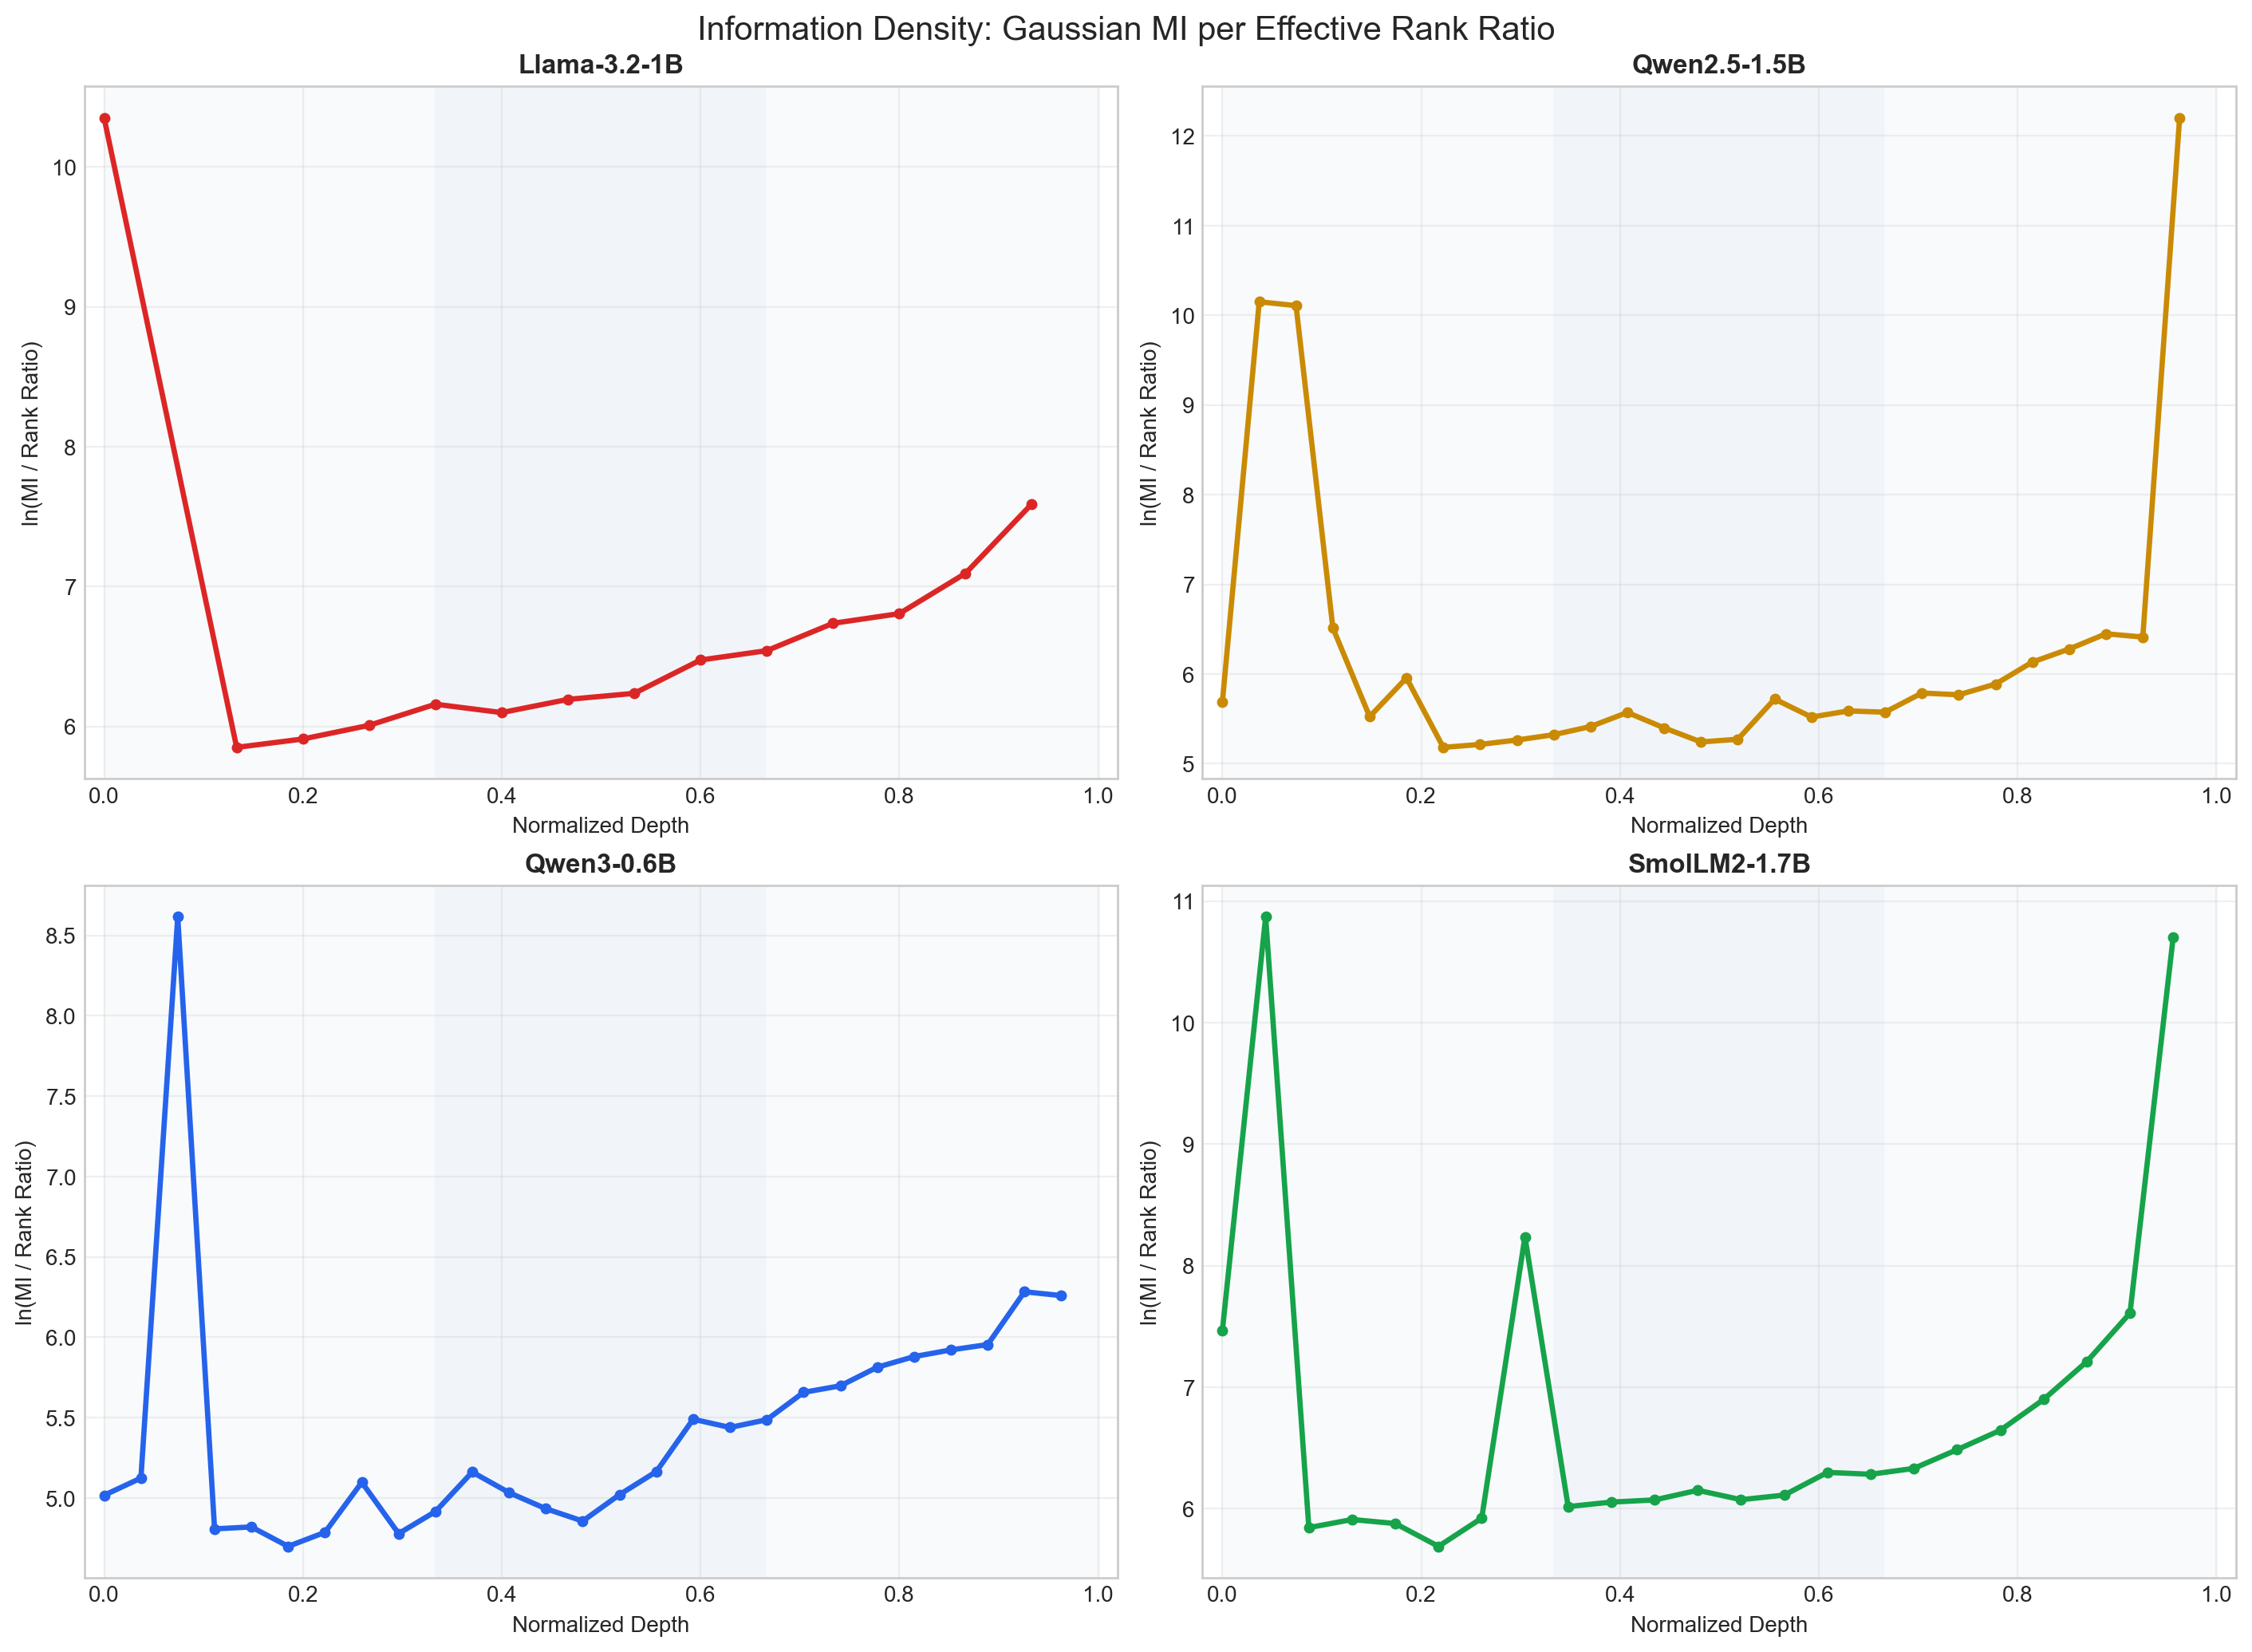
\includegraphics[width=0.85\textwidth]{result/7_information_plane/information_density.png}
\caption{Log information density $\rho_\ell = \ln(\mathrm{MI}_\ell / R_\ell)$ across normalized depth. All four models exhibit a U-shaped pattern.}
\label{fig:density}
\end{figure}

Across all four models, information density exhibits a \textbf{U-shaped pattern} (Figure~\ref{fig:density}):

\begin{itemize}
    \item \textbf{Rank-1 layers} ($\rho_\ell \approx 8$--$12$): One or two active dimensions carrying disproportionate output-relevant information. These are the most \emph{efficient} representations in the network---not redundancies, but learned bottlenecks.
    \item \textbf{Middle layers} ($\rho_\ell \approx 5$--$6$): Many active dimensions, each carrying little output-relevant information. These are the least efficient layers and the primary targets for compression.
    \item \textbf{Late layers} ($\rho_\ell$ rising from $\sim$6 to $\sim$8): Fewer dimensions than middle layers, but each increasingly aligned with the output. The network progressively concentrates information into a compact subspace.
\end{itemize}

This reframes rank-1 layers: rather than simply ``degenerate,'' they represent extreme information concentration. A single direction that carries $\rho_\ell > 10$ is a learned bottleneck---the network has discovered that this depth position benefits from radical compression.

\subsection{Pareto Efficiency Frontier}

\begin{figure}[h]
\centering
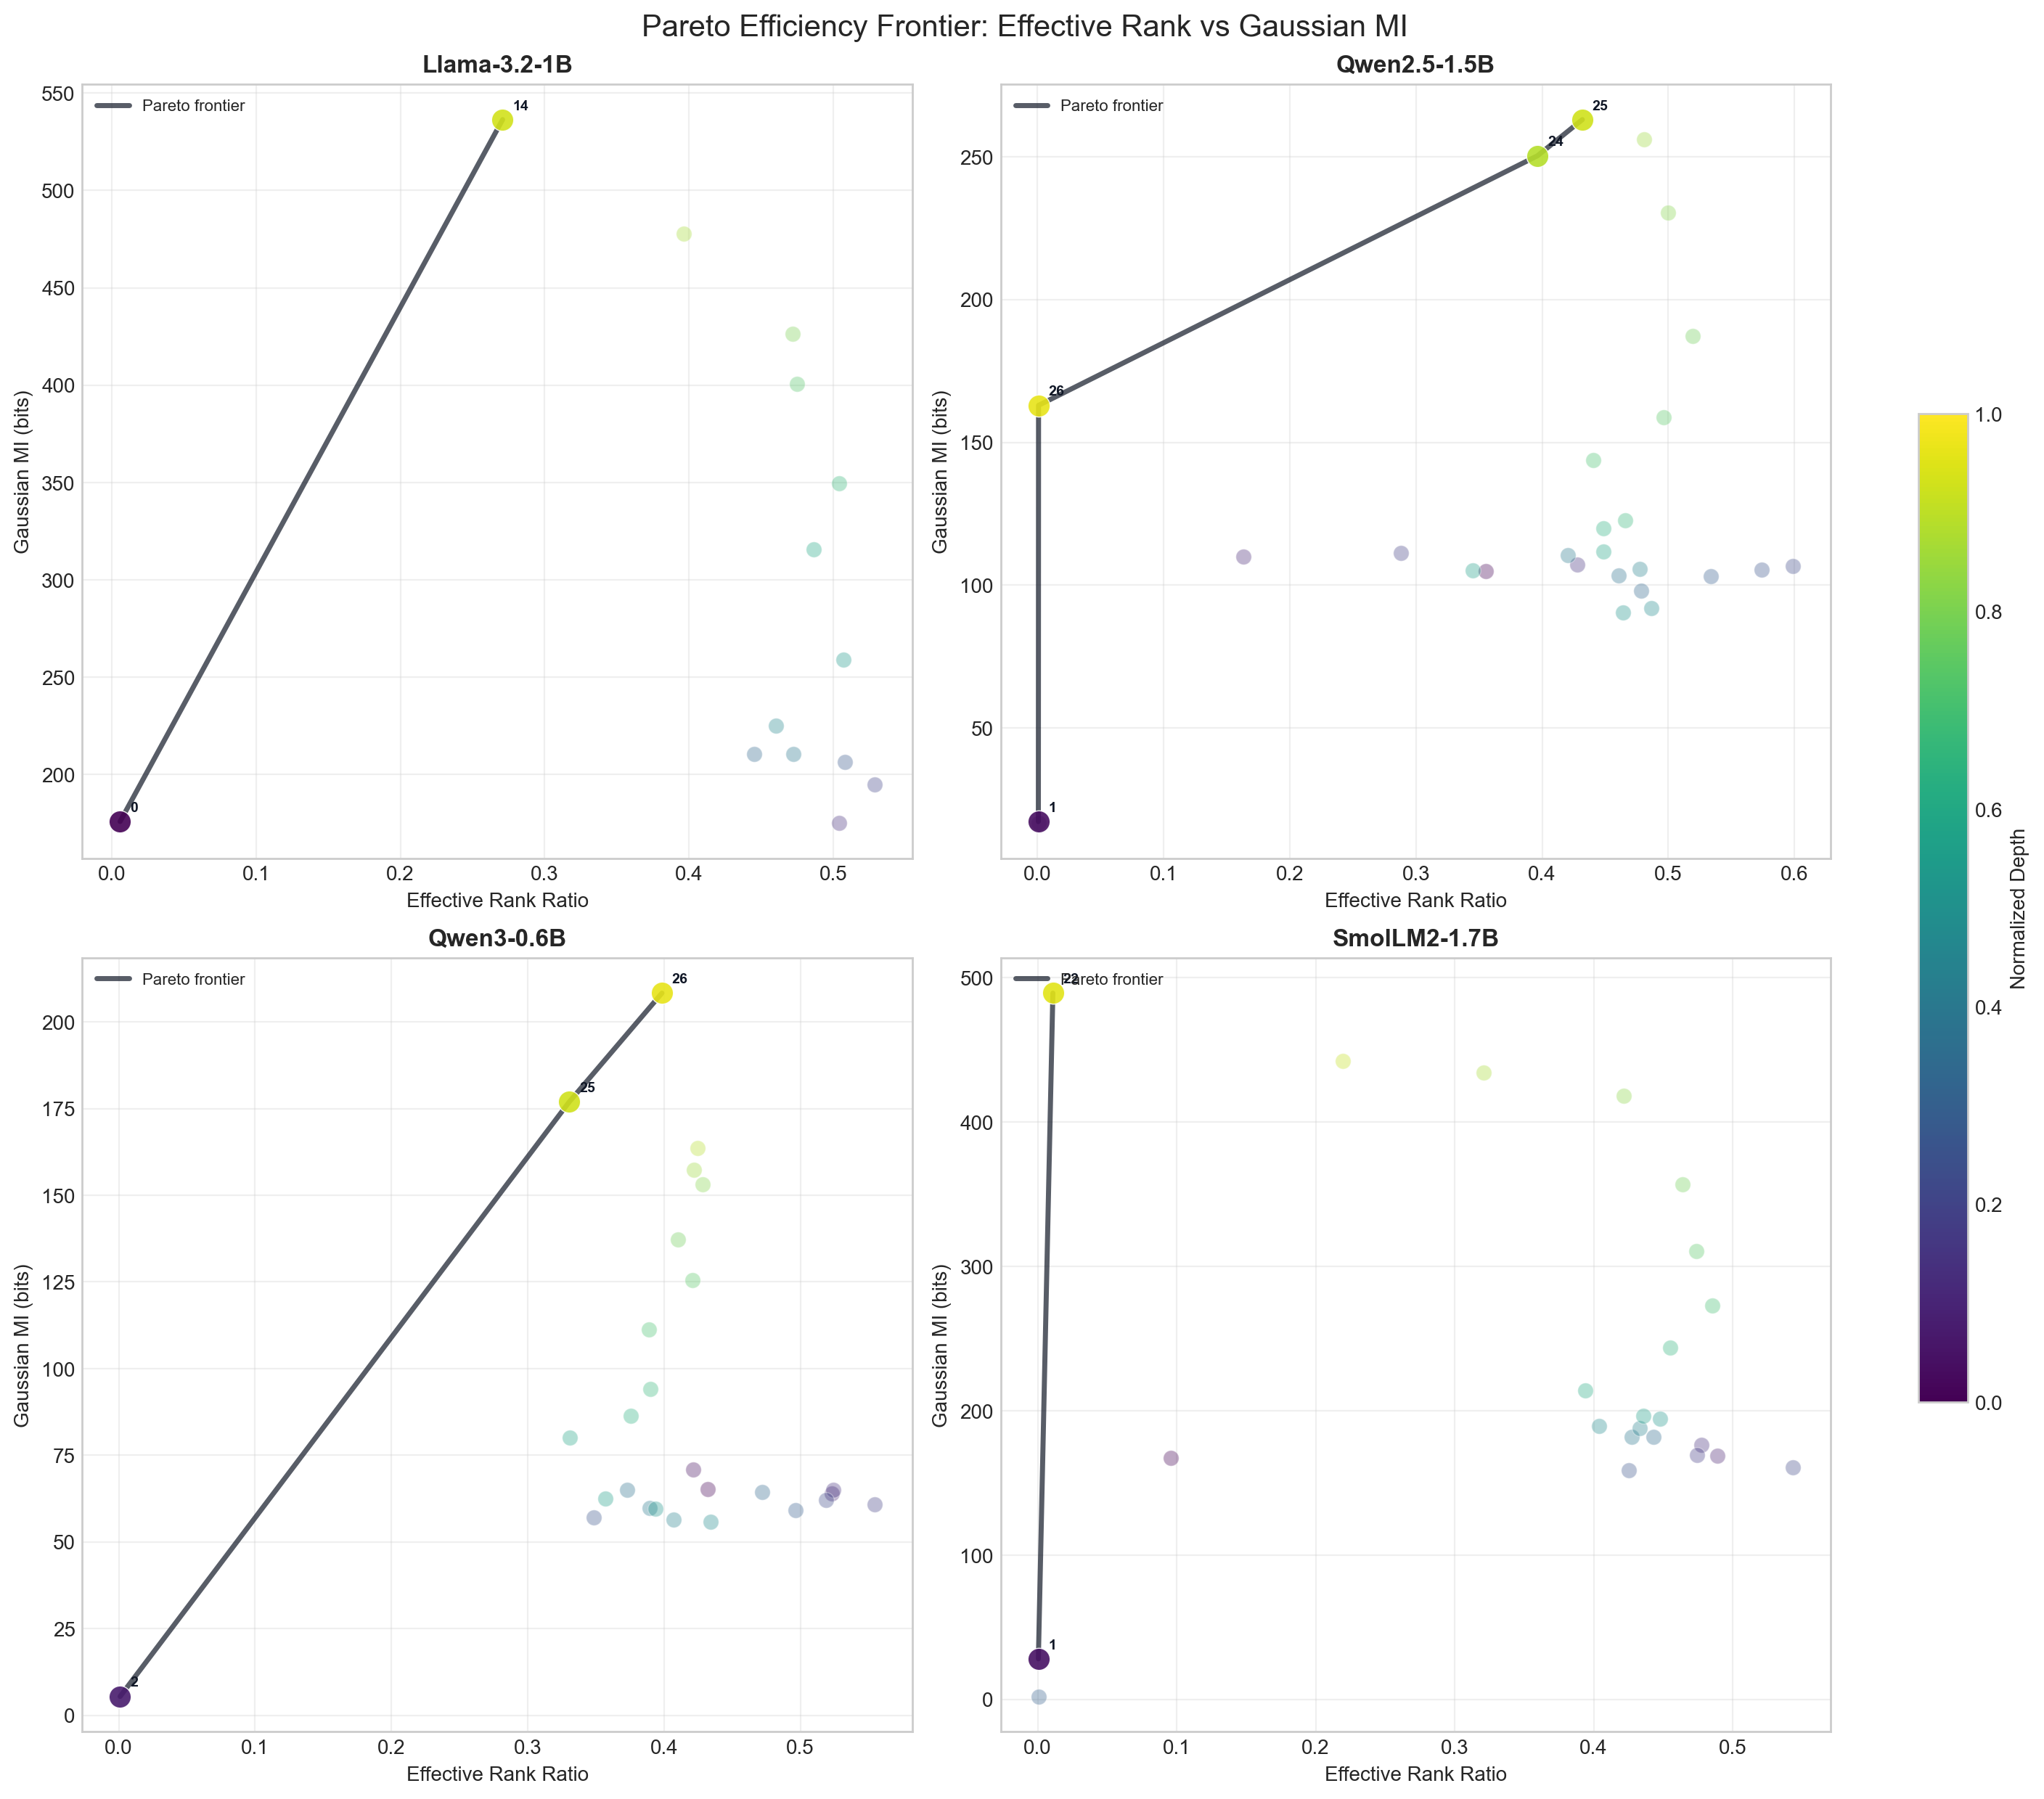
\includegraphics[width=0.85\textwidth]{result/7_information_plane/pareto_frontier.png}
\caption{Pareto frontier in (Effective Rank Ratio, Gaussian MI) space per model. Points colored by normalized depth (purple = early, yellow = late). Only 2--4 layers per model are non-dominated.}
\label{fig:pareto}
\end{figure}

We compute the Pareto frontier for each model: the set of layers where no other layer achieves both lower rank \emph{and} higher MI (Figure~\ref{fig:pareto}). Only \textbf{2--4 layers per model} lie on the frontier, consistently:
\begin{itemize}
    \item \textbf{Rank-1 layers}: minimal complexity, moderate-to-high MI depending on depth.
    \item \textbf{The final 1--2 layers}: highest MI with declining rank.
\end{itemize}
The remaining 80--90\% of layers are Pareto-dominated---they use more dimensions than necessary for the informativeness they achieve. This provides a quantitative, per-layer compression guide: dominated layers can be aggressively compressed; frontier layers should be preserved.

\subsection{Limitations}

These findings should be interpreted with the following caveats:
\begin{enumerate}
    \item \textbf{Proxy quantities.} Effective rank is a proxy for $I(T;X)$, not a direct measurement. Gaussian MI is a lower bound on true MI. The IB-like patterns we observe are \emph{consistent with} the Information Bottleneck principle, but we cannot claim that these models explicitly optimize the IB objective---standard training minimizes cross-entropy with no compression term.
    \item \textbf{Single dataset.} All results use WikiText-2 (65,536 tokens). Different domains may yield different patterns.
    \item \textbf{Small scale.} Models range from 0.6B to 1.7B parameters. Whether these patterns persist at 7B+ remains untested.
    \item \textbf{MLP only.} We analyze MLP outputs; attention heads also carry and transform information but are not included in this analysis.
    \item \textbf{$Y$ is proxied by the final layer.} The true target is next-token prediction; we use the final layer's MLP output as a proxy for $Y$.
\end{enumerate}

%% ================================================================
\section{Summary of My Contributions}
%% ================================================================

\begin{enumerate}
    \item \textbf{Gaussian MI pipeline} (scripts \texttt{6\_mutual\_information.py}, \texttt{6b\_mutual\_information\_residual.py}): Computes $I(\mathbf{m}_\ell;\, \mathbf{m}_L)$ for MLP output and $I(\mathbf{h}_\ell;\, \mathbf{h}_L)$ for residual stream via CCA (with truncated whitening) and log-det methods. Runs across all four models.

    \item \textbf{MLP vs.\ residual stream comparison} (script \texttt{6c\_mi\_comparison\_plot.py}): Dual-axis and normalized visualizations revealing the contrast between per-layer contributions and cumulative information flow.

    \item \textbf{Information plane analysis} (script \texttt{7\_information\_plane.py}): Combines effective rank ($I(T;X)$ proxy) with Gaussian MI ($I(T;Y)$ proxy) to place layers in the IB information plane. Includes scatter plots, depth-trend panels, Pareto efficiency frontier, and information density analysis.

    \item \textbf{Five empirical findings}:
    \begin{itemize}
        \item Two-phase MLP output MI with rank-1 drops (Section~\ref{sec:f1}).
        \item Smooth, monotonic residual stream MI consistent with DPI (Section~\ref{sec:f2}).
        \item The late-layer ``scissors''---compression--informativeness tradeoff (Section~\ref{sec:f3}).
        \item Universality across four architectures (Section~\ref{sec:f4}).
        \item U-shaped information density and Pareto frontier---rank-1 layers as learned bottlenecks, 80--90\% of layers dominated (Section~\ref{sec:f5}).
    \end{itemize}
\end{enumerate}

\bibliographystyle{plain}
\begin{thebibliography}{9}

\bibitem{tishby2015}
N.~Tishby and N.~Zaslavsky,
``Deep Learning and the Information Bottleneck Principle,''
\emph{IEEE Information Theory Workshop (ITW)}, 2015.
arXiv:1503.02406.

\bibitem{shwartz2017}
R.~Shwartz-Ziv and N.~Tishby,
``Opening the Black Box of Deep Neural Networks via Information,''
arXiv:1703.00810, 2017.

\bibitem{chechik2005}
G.~Chechik, A.~Globerson, N.~Tishby, and Y.~Weiss,
``Information Bottleneck for Gaussian Variables,''
\emph{Journal of Machine Learning Research}, 6:165--188, 2005.

\bibitem{roy2007}
O.~Roy and M.~Vetterli,
``The Effective Rank: A Measure of Effective Dimensionality,''
\emph{European Signal Processing Conference (EUSIPCO)}, 2007.

\end{thebibliography}

\end{document}
